\documentclass[reprint, aps, prx, amsmath, amssymb, longbibliography, superscriptaddress]{revtex4-2}

%% don't need amsmath because it is loaded in \documentclass
%% \usepackage{amsmath,amssymb}
\usepackage{graphicx}
\usepackage{epsfig}
\usepackage{mathrsfs,esint}
\usepackage{physics}
\usepackage{relsize}
%% \usepackage{float} %% revtex4-2 has a conflict with float
\usepackage{dsfont}
\usepackage{comment}
\usepackage{svg}

%% packages for combining several images into a single figure
%%\usepackage{caption}
%%\usepackage{subcaption}
\usepackage[caption=false]{subfig}

%% Hyperref loaded the last because some packages may redefine \label
\usepackage[bookmarks=true,
   colorlinks=true,
   linkcolor=blue,
   urlcolor=blue,
   citecolor=blue,
   bookmarks=true,
   hyperindex=true
]{hyperref}
%\usepackage{natbib}

\definecolor{mediumtealblue}{rgb}{0.0, 0.33, 0.71}
\newcommand{\jk}[1]{{\color{mediumtealblue}#1}}
\newcommand{\al}[1]{{\color{purple}#1}}
\newcommand{\dl}[1]{{\color{red}#1}}


\DeclareMathOperator{\Zn}{\mathbb{Z}_n}
\DeclareMathOperator{\Zthree}{\mathbb{Z}_3}
\DeclareMathOperator{\Ztwo}{\mathbb{Z}_2}
\DeclareMathOperator{\Id}{Id}
\DeclareMathOperator{\diag}{diag}
\DeclareMathOperator{\sgn}{sign}


\begin{document}

\title{From \texorpdfstring{$\Zthree$}{Z3} Rabi model to Potts model}

\author{Anatoliy I. Lotkov}
\affiliation{Department of Physics, University of Basel, Klingelbergstrasse 81, CH-4056 Basel, Switzerland}

\author{Valerii K. Kozin}
\affiliation{Department of Physics, University of Basel, Klingelbergstrasse 81, CH-4056 Basel, Switzerland}


\author{Denis V. Kurlov}
\affiliation{Department of Physics, University of Basel, Klingelbergstrasse 81, CH-4056 Basel, Switzerland}


\author{Jelena Klinovaja}
\affiliation{Department of Physics, University of Basel, Klingelbergstrasse 81, CH-4056 Basel, Switzerland}

\author{Daniel Loss}
\affiliation{Department of Physics, University of Basel, Klingelbergstrasse 81, CH-4056 Basel, Switzerland}

%%%%%%%%%%%%%%


\begin{abstract}
We study the $\Zthree$-symmetric Rabi models in this paper. In particular, we consider 1-mode and 2-mode variants of the $\Zthree$ Rabi model and determine their spectra. Next, we derive a mapping of the 2-mode $\Zthree$ Rabi model onto a qubit-boson ring. This mapping allows us to formulate a possible implementation of the $\Zthree$ Rabi model based on superconducting qubits and provides a context for the previously proposed optomechanical implementation. Furthermore, we propose a physical implementation of the $\Zthree$ Potts model via a chain of $\Zthree$ Rabi models coupled through nearest-neighbor interactions. Finally, we investigate the effects of the disorder on these systems.
\end{abstract}

\maketitle


\section{Introduction}


 $\Zn$-symmetric systems have attracted attention in integrable models, topological phases, and quantum information. in integrable systems research, the $\Zn$ symmetric Potts model plays an important role, being the non-trivial generalization of the simplest integrable systems like the Ising model or the XXZ model \cite{wu_potts_1982,fortuin_randomcluster_1972,temperley_relations_1971,baxter_new_1988}. $\Zn$ symmetry also arises in topological phases: parafermionic edge modes—generalizations of Majorana modes—inherit it naturally \cite{fendley_free_2013,fendley_parafermionic_2012, teixeira_edge_2022,alicea_topological_2016,cobanera_fock_2014}. Finally, $\Zn$ symmetry is useful for applied quantum technology, where qudit‑based processors extend the usual qubit paradigm \cite{wang_qudits_2020, kiktenko_single_2015, kiktenko_scalable_2020,proctor_quantum_2019,farinholt_ideal_2014,brylinski_universal_2001}. Besides, modern platforms for quantum computations, such as trapped ions or superconducting qubits, inherently possess more than 2 energy levels that can be used for the computation. And systems based on $n$-level qudits unavoidably bear $\Zn$ symmetry.

For the sake of simplicity, we focus on the $\Zthree$ case; all results generalize readily to $\Zn$ case. The main topic of this paper is the $\Zthree$ Rabi model. The usual $\Ztwo$ Rabi model being one of the simplest quantum models is ubiquitous in modern condensed matter physics \cite{braumuller_analog_2017, braak_integrability_2011,hwang_quantum_2015, chen_shortcuts_2021}. Hence, it is therefore natural to study its $\Zn$ generalization, which has recently drawn interest \cite{albert_quantum_2012, zhang_$z_n$_2014, sedov_chiral_2020}. We also discuss several variants of the $\Zthree$ Rabi model, their similarities and differences. 

In particular, the model exhibits behavior similar to the superradiant phase found in the ordinary Rabi model. While a formal proof remains open, we present evidence for the existence of this phase transition. In the relevant regime, the ground state becomes a $n$-fold generalization of the cat state. A renewed interest in cat state research has emerged due to its proposed application as a Quantum Error Correction Code \cite{vlastakis_deterministically_2013,malbouisson_highergeneration_1999,bergmann_quantum_2016,grimm_stabilization_2020}. Cat states based on a two-photon dissipation boson system were even proposed as a platform for fault-tolerant quantum computation \cite{guillaud_repetition_2019}. However, cat-state quantum error correction has focused on qubits. In this work, by achieving 3-fold cat states, we extend it to qudits by realizing $\Zthree$ cat states.

We then present a method to experimentally implement the $\Zthree$ Rabi model in variouis physical platforms, illustrated by superconducting qubits. To our knowledge, it is the first proposal to realize the $\Zthree$ Rabi model experimentally. We exploit discrete rotational symmetry of 1-dimensional finite systems with periodic boundary conditions as a source of $\Zn$ symmetry. We also discuss why more straightforward approaches to implement the $\Zn$ Rabi model do not work.

Next, a generalization of Hwang's proposal to build an Ising model by coupling a chain of $\Ztwo$ Rabi models \cite{hwang_largescale_2013} allows us to combine a chain of $\Zthree$ Rabi models into a $\Zthree$ Potts model. As far as we know, quantum Potts models are also yet to be implemented in the experiment, except by simulating on a universal quantum computer. However, recently another realization based on Josephson junctions was proposed \cite{wauters_engineering_2024}. Hence, we believe our proposal could be of interest. 

Additionaly, the Potts model is dual to a parafermion chain \cite{fradkin_disorder_1980}. In particular, the chiral Potts model, i.e., a chain of Rabi models coupled chirally, exhibits already mentioned parafermion edge modes \cite{fendley_free_2013,fendley_parafermionic_2012}. Although we only briefly touch on the parafermion edge modes in this paper, we believe that a further investigation in this direction could be fruitful.

In the remainder of the manuscript we proceed as follows. In Sec.~II, we introduce the 1-mode $\Zn$ and $\Zthree$ Rabi models and study their properties. Next, in Sec.~III, this construction is generalized to the 2-mode $\Zthree$ Rabi model. In Sec.~IV, the 2-mode $\Zthree$ Rabi model is mapped to a qubit-boson ring of length 3. It allows us to propose superconducting-circuit and optomechanical implementations of the model. In Sec.~V,  the nearest‑neighbour $\Zthree$ Potts model is built from a chain of $\Zthree$ Rabi models. In Sec.~VI we analyze the impact of the disorder on the proposed construction. We conclude in Sec.~VII.



\section{$\Zthree$ Rabi model.}


\subsection{Qubit--boson ring}
\label{physical-implementation}

In this section we demonstrate how the two--mode $\Zthree$ Rabi model emerges
in the single--excitation sector of a three--site qubit--boson (QB) ring with
nearest--neighbour coupling.  Superconducting and optomechanical
implementations are briefly commented on, while a compact derivation for a
general interaction matrix is deferred to
Sec.~\ref{arbitrary-interaction-summary}.  Throughout we follow the notation of the
main text and retain only the steps essential for the specific form of the
interaction.

The QB ring Hamiltonian is
\begin{equation}
\label{physical-hamiltonian}
  \begin{aligned}
    \hat H_{\text{QB}} &= \epsilon \sum_{j=0}^{2} \sigma_j^z
      + \Omega_{\text{QB}} \sum_{j=0}^{2} \hat a_j^{\dagger} \hat a_j
      + \hat V_{\text{QB}},
      \\
    \hat V_{\text{QB}} &= g \sum_{j=0}^{2}
      \bigl( \sigma_j^{+} \sigma_{j+1}^{-}
      e^{ i ( \hat x_j - \hat x_{j+1} ) } + \text{h.c.} \bigr),
  \end{aligned}
\end{equation}
where $\Omega_{\text{QB}}$ is the boson frequency and $m_{\text{QB}}$ the
effective mass.  Creation and annihilation operators are defined in the usual
way,
\begin{equation}
  \hat a_j = \sqrt{\frac{m_{\text{QB}} \Omega_{\text{QB}}}{2}}\, \hat x_j
           + i \sqrt{ \frac{1}{2 m_{\text{QB}} \Omega_{\text{QB}}} }\, \hat p_j.
\end{equation}
This is a variant of the model studied in
Ref.~\cite{sedov_chiral_2020}.

Because $[ \hat H_{\text{QB}}, \hat S^z ] = 0$ with $\hat S^z = \sum_j
\sigma_j^z$, the number of spin excitations is conserved.  We therefore focus
on the single--excitation subspace
\begin{equation}
  \mathcal H_{\text{QB},1} = \operatorname{Span}\bigl\{ |
    \uparrow\downarrow\downarrow\rangle,
    |\downarrow\uparrow\downarrow\rangle,
    |\downarrow\downarrow\uparrow\rangle \bigr\}.
\end{equation}

\paragraph{Spin--dependent momentum translation.}
Applying the unitary operator
$S = \prod_j e^{ i \sigma_j^z \hat x_j / 2 }$ removes the exponentials in
$\hat V_{\text{QB}}$ and yields
\begin{equation}
\label{after-momentum-translation}
  \begin{aligned}
    S^{-1} \hat H_{\text{QB}} S &= \epsilon \sum_{j} \sigma_j^z
      + \Omega_{\text{QB}} \sum_j \hat a_j^{\dagger} \hat a_j
      + \frac{1}{2 m_{\text{QB}}} \sum_j \hat p_j \sigma_j^z
      \\
      &\quad + \frac{3}{4 m_{\text{QB}}}
      + g \sum_{j}
        \bigl( \sigma_j^{+} \sigma_{j+1}^{-} + \sigma_j^{-} \sigma_{j+1}^{+} \bigr).
  \end{aligned}
\end{equation}
The qubit interaction is now purely spin--spin, at the price of an additional
spin--boson term proportional to $\hat p_j \sigma_j^z$.

\paragraph{Discrete Fourier transform.}
Introducing momentum--space operators $\hat a(k)$ and spin operators $S^{\pm}(k)$
via the unitary (type-I) discrete Fourier transform, $\hat a(k)= \tfrac{1}{\sqrt{3}}\sum_{j}e^{-2\pi i jk/3}\hat a_j$ (and analogously for the spins), we
bring Eq.~\eqref{after-momentum-translation} to
\begin{equation}
\label{after-fourier}
  \begin{aligned}
    &\hat H_{\text{FT}} = \epsilon \sum_{k=0}^{2} S^{z}(k)
      + \Omega_{\text{QB}} \sum_{k=0}^{2} \hat a^{\dagger}(k) \hat a(k)
                         + \frac{3}{4 m_{\text{QB}}} \\
     &+\frac{1}{2 m_{\text{QB}}} \sum_{k=0}^{2} \hat p(k) S^{z}(-k)
            + g \sum_{k=0}^{2} \bigl( S^{+}(k) S^{-}(-k) + \text{h.c.} \bigr),
  \end{aligned}
\end{equation}
which is block-diagonal in the crystal momentum $k$.

\paragraph{Restriction to $\mathcal H_{\text{QB},1}$.}
Inside the single--excitation subspace the zero-momentum ($k=0$) boson mode
decouples from the dynamics.  Discarding constants and the inert mode we obtain
\begin{equation}
  \begin{aligned}
    \hat H_{\text{QB},1} &= \Omega_{\text{QB}} \sum_{k=1}^{2} \hat a^{\dagger}(k)
      \hat a(k) + g \bigl( X + X^{\dagger} \bigr)
      \\
      &\quad + i \sqrt{ \frac{\Omega_{\text{QB}}}{6 m_{\text{QB}}} }
        \Bigl[ -( \hat a(1) - \hat a^{\dagger}(2) ) Z
        - ( \hat a(2) - \hat a^{\dagger}(1) ) Z^{\dagger} \Bigr].
  \end{aligned}
\end{equation}

\paragraph{Final rearrangement.}
A Hadamard transform on the spin degrees of freedom, combined with a global
bosonic $U(1)$ phase rotation, brings the Hamiltonian to the canonical
$\Zthree$ two--mode Rabi form,
\begin{equation}
\label{effective-rabi}
  \begin{aligned}
    \hat H_{\text{R}2} &= \Omega_{\text{QB}}
      \bigl( \hat a^{\dagger}(1) \hat a(1) + \hat a^{\dagger}(2) \hat a(2) \bigr)
      + g \bigl( Z + Z^{\dagger} \bigr)
      \\
      &\quad - \sqrt{ \frac{\Omega_{\text{QB}}}{6 m_{\text{QB}}} }
      \Bigl[ ( \hat a(1) + \hat a^{\dagger}(2) ) X
        + ( \hat a(2) + \hat a^{\dagger}(1) ) X^{\dagger} \Bigr].
  \end{aligned}
\end{equation}
The identification with Eq.~(\ref{2-mode-Z3-Rabi}) is
\begin{equation}
\label{QB-RM-parameter-mapping}
  \Omega_R = \Omega_{\text{QB}},
  \quad B = g,
  \quad \phi = 0,
  \quad \lambda = \sqrt{ \frac{\Omega_{\text{QB}}}{6 m_{\text{QB}}} }.
\end{equation}

For completeness we record the explicit ``magnetic'' term,
\begin{equation}
\label{superconducting-magnetic-term}
  g \bigl( Z + Z^{\dagger} \bigr) =
  \begin{pmatrix}
    2 g & 0 & 0 \\
    0 & -g & 0 \\
    0 & 0 & -g
  \end{pmatrix}.
\end{equation}
Thus the two--mode $\Zthree$ Rabi model faithfully captures the dynamics of
the QB ring in the single--excitation sector.

We emphasise superconducting qubits as a natural platform for engineering the
interaction~\eqref{physical-hamiltonian}, although analogous constructions are
possible in, for example, optomechanical settings.


\subsubsection{Why so complicated?}

The implementation of the $\Zthree$ Rabi model proposed in the previous section is considerably more complicated than the usual $\Ztwo$ Rabi model implementations. To obtain the $\Ztwo$ Rabi model it is enough to simply couple a qubit with a boson in a naive way. Therefore, one may wonder if these complications are needed. However, the straightforward generalization of the $\Ztwo$ Rabi model to higher Rabi models does not work due to fundamental obstacles. It turns out to be considerably more difficult to get a $\Zthree$ symmetric interaction. In this section, we try to explain why.

There are two most common ways to get a two-level quantum system. It is possible to use a spin as a $2$-level system  \cite{bosco_fully_2022,felicetti_quantum_2017,skogvoll_tunable_2021} or two levels in anharmonic oscillator, e.g., the Rabi model describes a superconducting qubit coupled to a cavity in the ultra-strong coupling regime \cite{niemczyk_circuit_2010,forn-diaz_ultrastrong_2017,yoshihara_superconducting_2017,vlasiuk_cavityinduced_2023, kozin_quantum_2024,chen_singlephotondriven_2017,PhysRevA.106.023702}. Therefore, it is simple to get a $\Ztwo$ Rabi model. It is enough to take either a spin or an anharmonic oscillator and couple it to a boson mode using $\hat V = \sigma_x \hat x_{\text{boson}}$.

Both ways are easily generalized to the $\Zthree$ Rabi model. To get a spin-based 3-level system we just need to take spin $1$. However, in this case, we obtain an interaction through the spin-1 representation of $s^x$ instead of $X$.
\begin{equation}
    s^x= \begin{pmatrix} 0 & \sqrt{2} & 0 \\ \sqrt{2} & 0 & \sqrt{2} \\ 0 & \sqrt{2} & 0 \end{pmatrix}
\end{equation}
It is easy to see that it is not $\Zthree$-symmetric. Hence, the spin $1/2$ representation of the $SU(2)$ group is a convenient special case that, unfortunately, does not generalize. It does not mean that it is impossible to build a $\Zthree$ symmetric system out of spins as we have shown, or higher $\Zn$ symmetric systems \cite{hutter_parafermions_2015} in general. But it still explains why we need rather complicated ways to achieve it.

The second way to get a $\mathbb{Z}_2$ Rabi model is to use $2$ levels of an anharmonic oscillator. Consequently, in the $\mathbb{Z}_2$ case $\sigma^x$ operator is basically a restriction of the coordinate operator  of the anharmonic oscillator $ \hat x_{\text{an}} = (\hat a_{\text{an}} + \hat a_{\text{an}}^{\dagger})/\sqrt{2} $ to the two lowest levels. On the contrast, if we restrict it to 3-level system, we get
\begin{equation}
    \hat x_{\text{an}} = \frac{1}{\sqrt{2}}\begin{pmatrix} 0 & \sqrt{1} & 0 \\ \sqrt{1} & 0 & \sqrt{2} \\ 0 & \sqrt{2} & 0 \end{pmatrix}
\end{equation}
As a result, the $\Ztwo$ Rabi model based on the anharmonic oscillator does not generalize to the higher $\Zn$ Rabi models.

These obstacles make an experimental $\Zn$‑Rabi realization non‑trivial, motivating our proposal.

The rationale provided in this section is in no way a formal proof. However, the argument should serve as an intuition as to why $\Zthree$ Rabi is less straightforward to engineer than its more well-known analogue. The model we proposed in the previous section solves this problem by having an inherent $\Zthree$ symmetry. It originates from the translational symmetry of a ring.

\subsection{Superconducting circuit implementation}
\label{superconducting-implementation}


The obvious choice for boson modes is an LC circuit. For the qubit ($\sigma_i$)  we consider superconducting charge qubits \cite{bouchiat_quantum_1998,nakamura_coherent_1999,lehnert_measurement_2003,makhlin_quantumstate_2001}, because we want the qubit eigenstate to be a charge state. More extensive discussion on the charge qubits we use is provided in App. \ref{charge-qubit}. Here, we only want to comment that the qubit eigenstates are $|0\rangle, |1\rangle$ defined by $\hat n |0\rangle = 0, \, \hat n |1\rangle = |1\rangle$, where $\hat n$ is the capacitor charge operator. Below, to denote a linear span of these states we use $\mathcal{V}_k = \operatorname{Span}\{|0\rangle_k, \, |1\rangle_k\}$ where $k$ is the number of the qubit.

Fig.~\ref{fig:superconducting-Rabi} shows a superconducting realization of the three‑site qubit–boson ring. Each horizontal branch of the circuit (Fig.~\ref{fig:superconducting-Rabi}) correspond to site $i = 0,1,2$ of the qubit-boson ring. The $i$th boson and qubit are implemented by the LC circuit and SC qubit on the $i$th branch respectively. The JJs on the on the vertical segments of the circuit on the right of Fig.~\ref{fig:superconducting-Rabi} are responsible for the interaction term in $H_{QB}$~\eqref{physical-hamiltonian} \cite{siewert_aspects_2000,rasmussen_controllable_2019,shafranjuk_twoqubit_2006,allman_tunable_2014,hu_controllable_2007}. On Fig.~\ref{fig:superconducting-Rabi} is, the characteristic parameters of every circuit element are also shown: LC circuit's conductor and inductor have capacitance $C_{\text{B}}$ and inductance $L_{\text{B}}$ respectively. The qubit's JJ and capacitance have critical current $I_{\text{Q}}$ and capacitance $C_{\text{Q}}$ respectively. The coupling JJs on the right have critical current $I_{\text{R}}$. For clarity, we omit any elements that are necessary for an actual experimental implementation, e.g., read‑out resonators, flux‑bias lines, and filtering components.

\begin{figure}[t]
  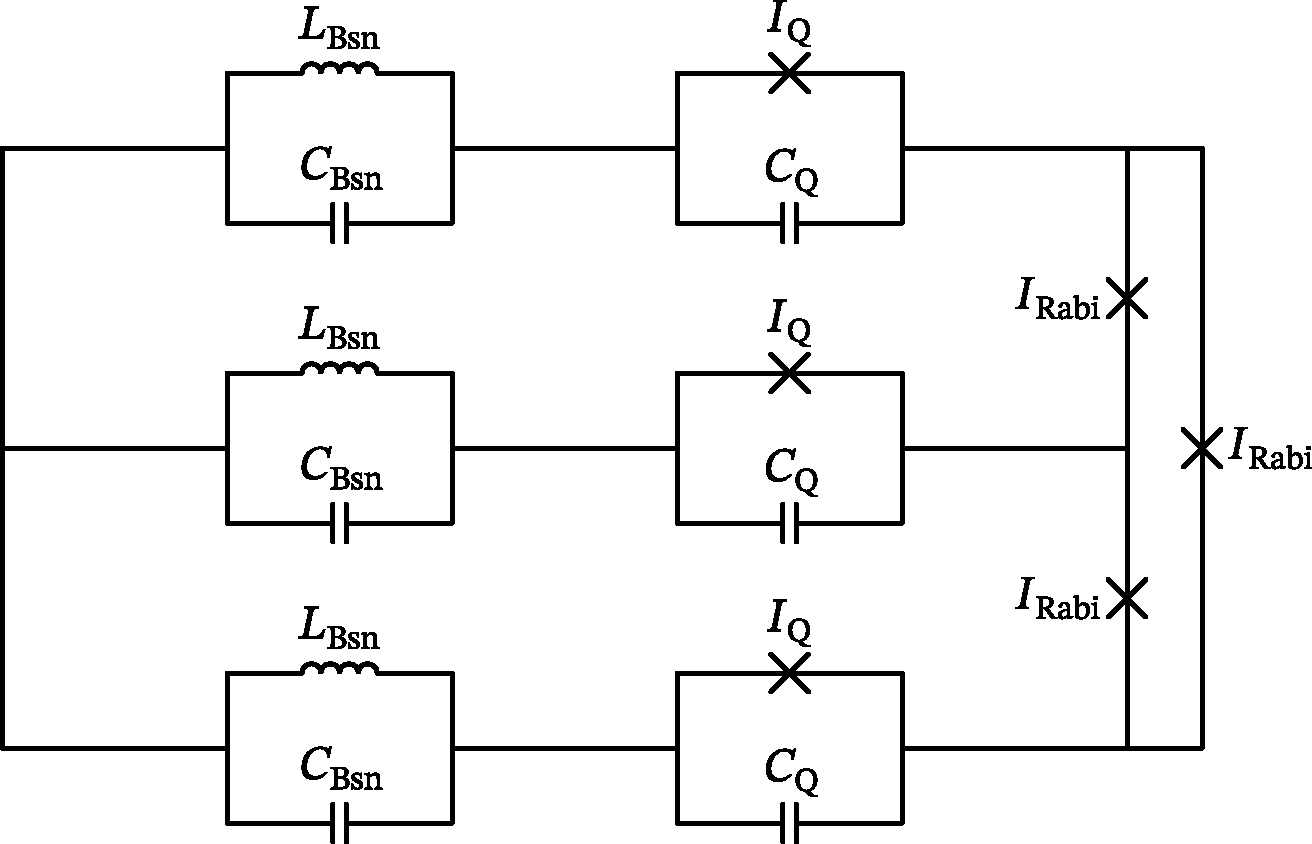
\includegraphics[width=\linewidth]{pics/SC_Rabi_circuit_svg-tex.pdf}
  \caption{Superconducting circuit implementation of the 2-mode $\Zthree$ Rabi model $\hat H_{\text{R}2}$. The LC circuits $(L_{\text{B}}, C_{\text{B}})$ host the boson modes; the charge qubits $(I_{\text{Q}}, C_{\text{Q}})$ correspond to the qubit degrees of freedom; Josephson junctions $I_{\text{Rabi}}$ are responsible for the interaction term in the qubit-boson ring. Altogether, the circuit is described by the Hamiltonian (\ref{physical-hamiltonian}).}
  \label{fig:superconducting-Rabi}
\end{figure}

Next, we describe why this circuit models the Hamiltonian~\eqref{physical-hamiltonian}. Without the coupling JJs, the LC circuits and qubits are independent from each other and are described by a non-interacting Hamiltonian:
\begin{equation}
  \hat H = \sum_{i = 0}^2 \hat H_{LC, i}(\phi_i, q_i) + \sum_{i = 0}^2 \hat H_{Q,i}(\varphi_i, n_i),
\end{equation}
where $ \phi_i, q_i$ are the magnetic flux and the capacitor charge of the $i$th LC circuit, while $\varphi_i, n_i$ are the JJsuperconducting phase and capacitor charge of the qubit. The LC circuit Hamiltonian is obviously $ H_{LC, i} = q_i^2/(2C) + \phi_i^2/(2L)$. Meanwhile, we leave the qubit Hamiltonian $\hat H_{Q,i} $ generic to allow different qubit types. However, we require the qubit to be a charge qubit and satisfy the following properties:
\begin{align}
   \hat H_{Q}\bigg|_{\mathcal{V}} = \begin{pmatrix} \bra{0_i}\hat H_Q\ket{0_i} & \bra{0_i} \hat H_Q \ket{1_i} \\ \bra{1_i} \hat H_Q \ket{0_i} & \bra{1_i} \hat H_Q \ket{1_i} \end{pmatrix} = \epsilon \sigma_z,
\end{align}
where the qubit states $\ket{0_i},\ket{1_i}$ are the charge operator eigenstates $ \hat q_i \ket{0_i} = Q \ket{1_i}, \, \hat q_{i} \ket{1}_i = (Q+1)\ket{1}_i$ with $ Q \in \mathbb{Z}$. $\mathcal{V}_i = \operatorname{Span}\{\ket{0_i},\, \ket{1_i}\}$ is a qubit Hilbert space, i.e, a computational subspace of the full Hilbert space of the qubit system $ \hat H_{Q,i}$. Due to this property, the operator $ e^{i\varphi_i} $ acts on the qubit subspace $\mathcal{V}_i$ as a raising operator:
\begin{equation}
  \begin{aligned}
    &e^{i\hat\varphi_i}\bigg|_{\mathcal{V}_i} = \begin{pmatrix} \bra{0_i} e^{i\hat\varphi_i} \ket{0_i} & \bra{0_i} e^{i\hat\varphi_i} \ket{1_i} \\ \bra{1_i} e^{i\hat\varphi_i} \ket{0_i} & \bra{1_i} e^{i\hat\varphi_i} \ket{1_i} \end{pmatrix} = \sigma^+,
  \end{aligned}
\end{equation}
because $[e^{i\phi}, n] = e^{i\phi}$.

If we now connect the $i$th and $(i+1)$th circuit branches with a JJ, it creates a cycle in the circuit. As a result, the fluxes and the superconducting phases have to satisfy a requirement:
\begin{equation}
  \hat \phi_i + \hat\varphi_i + \hat\varphi_R - \hat\varphi_{i+1} - \hat\phi_{i+1} = 2\pi N, \, \text{where}\ N \in \mathbb{Z}.
\end{equation}
In other words, the superconducting phase $\phi_R$ of the coupling JJ is not an independent degree of freedom. Therefore, for the corresponding term in the Hamiltonian we obtain:
\begin{equation}
    \hat V_{\text{SC QB},j} = I_{\text{R}} \cos(\hat \phi_R) =  I_{\text{R}}\cos(\hat \phi_j + \hat \varphi_j - \hat \phi_{j+1} - \hat \varphi_{j+1}).
\end{equation}


As we are only interested in qubit states $|0\rangle_k,\, |1\rangle_k$, we restrict the JJ term $\hat V_{\text{SC QB},j}$ to the qubit Hilbert subspace $\mathcal{V}_j\otimes \mathcal{V}_{j+1}$:
\begin{equation}
\begin{aligned}
    &\hat V_{\text{SC QB},j} \bigg |_{\mathcal{V}_j\otimes \mathcal{V}_{j+1}} = \\
    &=\frac{I_{\text{Rabi}}}{2}\left(e^{i(\hat\varphi_j - \hat\varphi_{j+1})} e^{i(\hat\phi_j - \hat\phi_{j+1})} + h.c. \right) \bigg|_{\mathcal{V}_j\otimes \mathcal{V}_{j+1}} \\
    &=\frac{I_{\text{Rabi}}}{2}\left(e^{i(\hat\varphi_j - \hat\varphi_{j+1})} \sigma_j^- \sigma_{j+1}^+ + h.c. \right).
\end{aligned}
\end{equation}
Here we used the fact that $e^{\pm i\hat\phi}$ acts as a raising/lowering operator for the charge qubit: $e^{i\hat\phi}|_{\mathcal{V}} = \sigma^+$. Hence the need for charge qubits rather than flux or phase qubits.

The Josephson junction coupling between two pairs of an LC circuits and a charge qubits gives us precisely the interaction term we wanted. As a result, we conclude that the system depicted in Fig. \ref{fig:superconducting-Rabi} is described by the Hamiltonian (\ref{physical-hamiltonian}).  The qubit-boson ring couplings can be expressed by the circuit parameters:
\begin{equation}
\begin{aligned}
    &\epsilon = \frac{\delta}{2 C_Q},\,
    \Omega_{QB} = \left(\sqrt{L_{\text{B}}C_{\text{B}}}\right)^{-1/2}, \\
    &m_{QB} = C_{\text{B}}, \, g = \frac{I_{\text{Rabi}}}{2}.
\end{aligned}
\end{equation}
For details of the $\epsilon$ computation, see App. \ref{charge-qubit}. Finally, applying Sec. $\ref{physical-implementation}$ argument we deduce that the circuit is described by the $\Zthree$ Rabi model.


\subsection{Optomechanical implementation}
\label{optomechanical-implementation}

\begin{figure}
    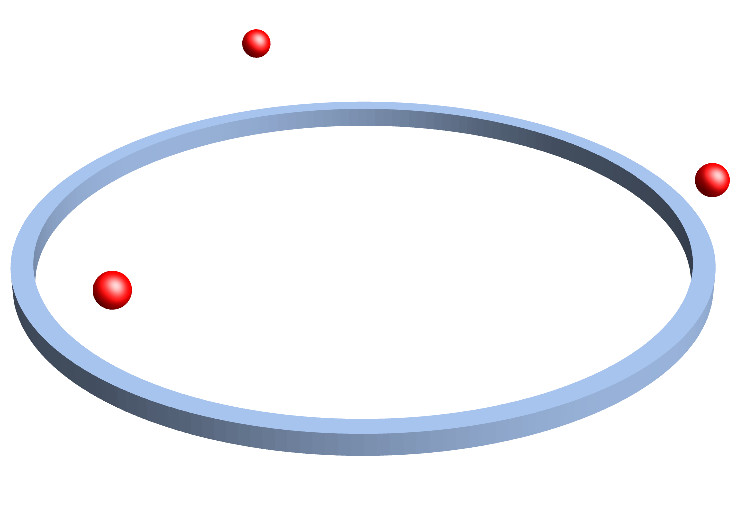
\includegraphics[width=0.8\linewidth]{pics/optomechanical_Rabi_pic.pdf}
    \caption{Schematic illustration of the optomechanical implementation of the 2-mode $\Zthree$ Rabi model $\hat H_{\text{R}2}$ \cite{sedov_chiral_2020} The red spheres are trapped ions carrying two-level systems; their vibrational modes are the bosons from the qubit-boson ring. The blue ring is the chiral waveguide that facilitates the interaction in the qubit-boson ring. The system is described by the Hamiltonian $\hat H_{\text{OM}}$ (\ref{optomechanical-qb-ring}).}
    \label{fig:optomechanical-rabi}
\end{figure}

Another possible physical platform for the $\Zthree$ Rabi model is an optomechanical system consisting of 3 spins whose vibrational modes are boson degrees of freedom. They are connected by a circular waveguide that acts as an interaction medium between the spins and the vibrational phonons (first proposed in \cite{sedov_chiral_2020}). 

Although challenging to realize, this platform illustrates the generality of our approach. In this section, we outline how the $\Zthree$ Rabi model arises in this model, for the extended discussion we refer the reader to the original paper \cite{sedov_chiral_2020}. 

The optomechanical model in question is described by the following Hamiltonian:
\begin{equation}
\label{optomechanical-qb-ring}
\begin{aligned}
    &\hat{H}_{\text{OM}}=\sum\limits_{j=0}^2 \zeta_j \hat{c}_j^{\dagger} \hat{c}_j + 
 \epsilon \sum_{j=0}^2 \sigma_j^z + \Omega_{\text{OM}} \sum_{j=0}^2 \hat{a}_j^{\dagger} \hat{a}_j + \hat{V}_{\text{int}}, \\
    &\hat{V}_{\text{int}}=\gamma \sum_{k, j=0}^2 \left[\sigma_j^{+} \hat{c}_k e^{i k\left[R \phi_j+\hat x_j\right]}+\text {h.c.}\right] \text {, }
\end{aligned}   
\end{equation}
where $\zeta_k = v k$.

Using the Schrieffer-Wolff transformation \cite{bravyi_schrieffer_2011}, we can integrate out the photons degrees of freedom to get the Hamiltonian in the form we want:

\begin{equation}
\begin{aligned}
&\hat{H}_{\text{OM,eff}}=  \epsilon \sum_j \sigma_j^z + \Omega_{\text{OM}} \sum_j \hat{a}_j^{\dagger} \hat{a}_j \\
& -\frac{\gamma^2}{2v} \sum_{i<j}\left[i \sigma_i^{+} \sigma_j^- e^{i q R \phi_{i j}} e^{i \eta\left(\hat{a}_i+\hat{a}_i^{\dagger}-\hat{a}_j-\hat{a}_j^{\dagger}\right)}+\text {h.c.}\right].
\end{aligned}
\end{equation}
The Hamiltonian is a bit different from (\ref{physical-hamiltonian}). It is treated in App. \ref{arbitrary-interaction} and gives rise to the following $\Zthree$ Rabi model:
\begin{equation}
\begin{aligned}
    &\hat H_{\text{2\:Rabi,mod}}= - \frac{\gamma^2}{2v} (e^{-5\pi i/6} Z + e^{5\pi i/6} Z^{\dagger}) \\
    &+ \Omega_{\text{OM}} (\hat a_1^{\dagger} \hat a_1 + \hat a_2^{\dagger} \hat a_2) \\
    &- \frac{\Omega_{\text{OM}}^{1/2} \eta}{6^{1/2}}\left[(\hat a_1 + \hat a_2^{\dagger}) X  + (\hat a_2 + \hat a_1^{\dagger}) X^{\dagger}  \right]
\end{aligned}
\end{equation}
which differs from the $\Zthree $ Rabi model we acquired in the superconducting circuit context only by the $\Zthree$ ``magnetic'' term's phase $\varphi = - 5\pi/6$.

We can explicitly write down the ``magnetic'' term
\begin{equation}
    - \frac{\gamma^2}{2v} (e^{-5\pi i/6} Z + e^{5\pi i/6} Z^2) = \begin{pmatrix}
        \frac{\sqrt{3}\gamma^2}{2v} & 0 & 0 \\ 0 & -\frac{\sqrt{3}\gamma^2}{2v} & 0 \\ 0 & 0 & 0 
    \end{pmatrix}.
\end{equation}
As one can see, the non-zero ``magnetic'' term's phase $\varphi$ leads to all the eigenvalues being non-degenerate. Compare it to Eq. (\ref{superconducting-magnetic-term}).




\section{\texorpdfstring{$\Zthree$}{Z3} Potts model}
\label{potts-model}

\subsection{Theoretical description}
\label{theoretical-potts}


The $\Zthree$ Potts model \cite{wu_potts_1982} is a 1-dimensional chain of $3$-level systems with a global $\Zthree$ symmetry. It  originates from statistical physics as a straightforward generalization of the Ising model to more states on each site \cite{wu_potts_1982,baxter_critical_1982}. Nowadays, the Potts model often appears in the context of qudit quantum computations \cite{aharonov_polynomial_2007,okada_efficient_2019}. However, the direct experimental realization of the Potts model still does not exist. One of the goals of this paper is to propose such an experimental realization based on $\Zthree$ Rabi models. To achieve this, we generalize the idea of building an Ising model by coupling a chain of $\Ztwo$ Rabi models, proposed by Hwang \cite{hwang_largescale_2013}, to the $\Zthree$-symmetric case.

The $\Zthree$ Potts model Hamiltonian is
\begin{equation}
\begin{aligned}
\label{potts-hamiltonian}
  \hat H_{\text{Potts}} =& f_{\text{Potts}} \sum\limits_{n=1}^L \left(e^{i\phi}Z_n + e^{-i\phi}Z_n^{\dagger}\right) \\
  &+  J_{\text{Potts}} \sum\limits_{n=1}^L \left( X_n X_{n+1}^{\dagger} + X_n^{\dagger} X_{n+1}\right). 
\end{aligned}
\end{equation}
The first term just describes single-excitation energies, the second term is the $\Zthree$-symmetric nearest-neighbour interaction.

As we already discussed before, it is difficult to obtain a $\Zthree$ symmetry in an arbitrary $3$-level system chain. But we have already learnt how to build a $\Zthree$ Rabi model. We use it as a building block for the $\Zthree$ Potts model, i.e., we want the 3 cat-states in the $\Zthree$ Rabi models (\ref{three-cat-states}) to serve as 3 states on the $n$th site of the Potts model $ |j\rangle_n = |\psi_j\rangle_n $ for $j=0,\, 1,\, 2$. By raising boson energy $\Omega_R$ in the Rabi model Hamiltonian (\ref{2-mode-Z3-Rabi}) the higher energy states are effective decoupled from $|\psi_j\rangle$ states.

The main reason why it is convenient to build the Potts model from Rabi models is that the boson degrees of freedom in the Rabi models allow us to obtain a $\Zthree$ symmetric interaction. The reasoning is simple; the Rabi model's $\Zthree$ symmetry acting on bosons is a residue of a usual $U(1)$ boson symmetry. Consequently, if we take a $U(1)$ symmetric interaction of boson modes on neighbor sites, then it is by default be $\Zthree$ symmetric. And the simplest $U(1)$ symmetric boson interaction is just a hopping term $\hat a_n^{\dagger} \hat a_{n+1} + \textrm{h.c.}$ As a result, to obtain a $\Zthree$ Potts model we need to take a chain of $\Zthree$ Rabi models and couple them by the boson hopping term:
\begin{equation}
\label{coupled-rabi}
\begin{aligned}
    &\hat H_{\text{Rabi chain}} = \\
    &\sum\limits_{n=1}^L \hat H_{\text{Rabi}, n} + J \sum\limits_{n=1}^L \sum\limits_{k=1}^2\left( \hat a_{n,k}^{\dagger} \hat a_{n+1,k} + \hat a_{n+1,k}^{\dagger} \hat a_{n,k}\right),
\end{aligned}
\end{equation}
where $n$ is a chain-site subscript and $k$ is a number of a boson mode in a $ \Zthree $ Rabi model. We claim that this Hamiltonian gives us precisely the $\Zthree$ Potts model, when we restrict it to the Hilbert space $\bigotimes_n\mathcal{R}_n$ generated by the 3 cat states on the sites $n=1,\dots,L$.

Within the Rabi qutrit subspace,  $\hat a_{n,k}$ acts as a permutation between the cat states:
\begin{equation}
    \hat a_{n,k} |\psi_i\rangle_n = (\lambda/\Omega)|\psi_{i+1}\rangle_n. 
\end{equation}

For the creation operator it is a little bit more complicated:
\begin{equation}
\begin{aligned}
    &\hat a_{n,k}^{\dagger} |\psi_i\rangle_n =  (\lambda/\Omega)|\psi_{i-1}\rangle_n + \delta, \,\text{where} \\
    &|\delta|^2 = 1.
\end{aligned}
\end{equation}
In the deep-strong coupling~\cite{PhysRevB.111.035410,kozin2025schottkyanomalycavitycoupleddouble} regime $\lambda/\Omega \gg 1$, we can neglect $\delta$. As a result, in the Rabi qutrit subspace the creation/annihilation operators act as cyclic permutations: $\hat a_{n,k}|_{\mathcal{R}} = (\lambda/\Omega) X$, $\hat a_{n,k}^{\dagger}|_{\mathcal{R}} = (\lambda/\Omega) X^{\dagger}$. Consequently, in this sector the coupled Rabi chain is equivalent to the Potts model:

\begin{equation}
\begin{aligned}
    J &\sum\limits_{k=0}^{2} \left(\hat a_{n,k}^{\dagger} \hat a_{n+1,k} + \hat a_{n+1,k}^{\dagger} \hat a_{n,k}\right) = \\
    &3(\lambda/\Omega)^2 J\left(X_n^{\dagger} X_{n+1} + X_{n+1}^{\dagger} X_n\right).
\end{aligned}
\end{equation}
Therefore, we have $J_{\text{Potts}} = 3(\lambda/\Omega)^2 J$.


\subsubsection{Underlying qubit-boson ring}

Considering that the Rabi models in the chain are made from a qubit-boson ring, we need to show how to obtain the boson hopping interaction (\ref{coupled-Rabi}) in terms of the QB ring degrees of freedom.

It turns out to be quite simple. If we add hopping terms for the bosons in the qubit-boson chain, then it gives us the hopping term between the Rabi model bosons, because the Fourier transform does not change the form of the boson hopping interaction:
\begin{equation}
\begin{aligned}
    &\sum\limits_{j=0}^2 \left(\hat a_{n,j}^{\dagger} \hat a_{n+1,j} + \hat a_{n+1,j}^{\dagger} \hat a_{n,j}\right) \\
    &=\sum\limits_{k=0}^{2} \left(\hat a_{n,k}^{\dagger} \hat a_{n+1,k} + \hat a_{n+1,k}^{\dagger} \hat a_{n,k}\right)
\end{aligned}
\end{equation}
To simplify the notation, we do not use brackets here to denote the Fourier components of the boson modes. The subscript $j$ correspond to the real space boson mode; the subscript $k$ corresponds to the Fourier boson mode, i.e., the $\Zthree$ Rabi model boson modes. We have an extra term $\hat a_{n,0}, \hat a^{\dagger}_{n,0}$ which decouples the same way it did in Sec. \ref{physical-implementation}.

The mapping between the parameters is the following:
\begin{equation}
\begin{aligned}
    &f_{\text{Potts}} = g \exp\left(-\frac{1}{2 m_{QB} \Omega_{QB}}\right),\\
    &J_{\text{Potts}} = \frac{J }{2 m_{QB} \Omega_{QB}} .
\end{aligned}
\end{equation}

\subsection{Coupled superconducting \texorpdfstring{$\Zthree$}{Z3} Rabi models}


\begin{figure}[t]
    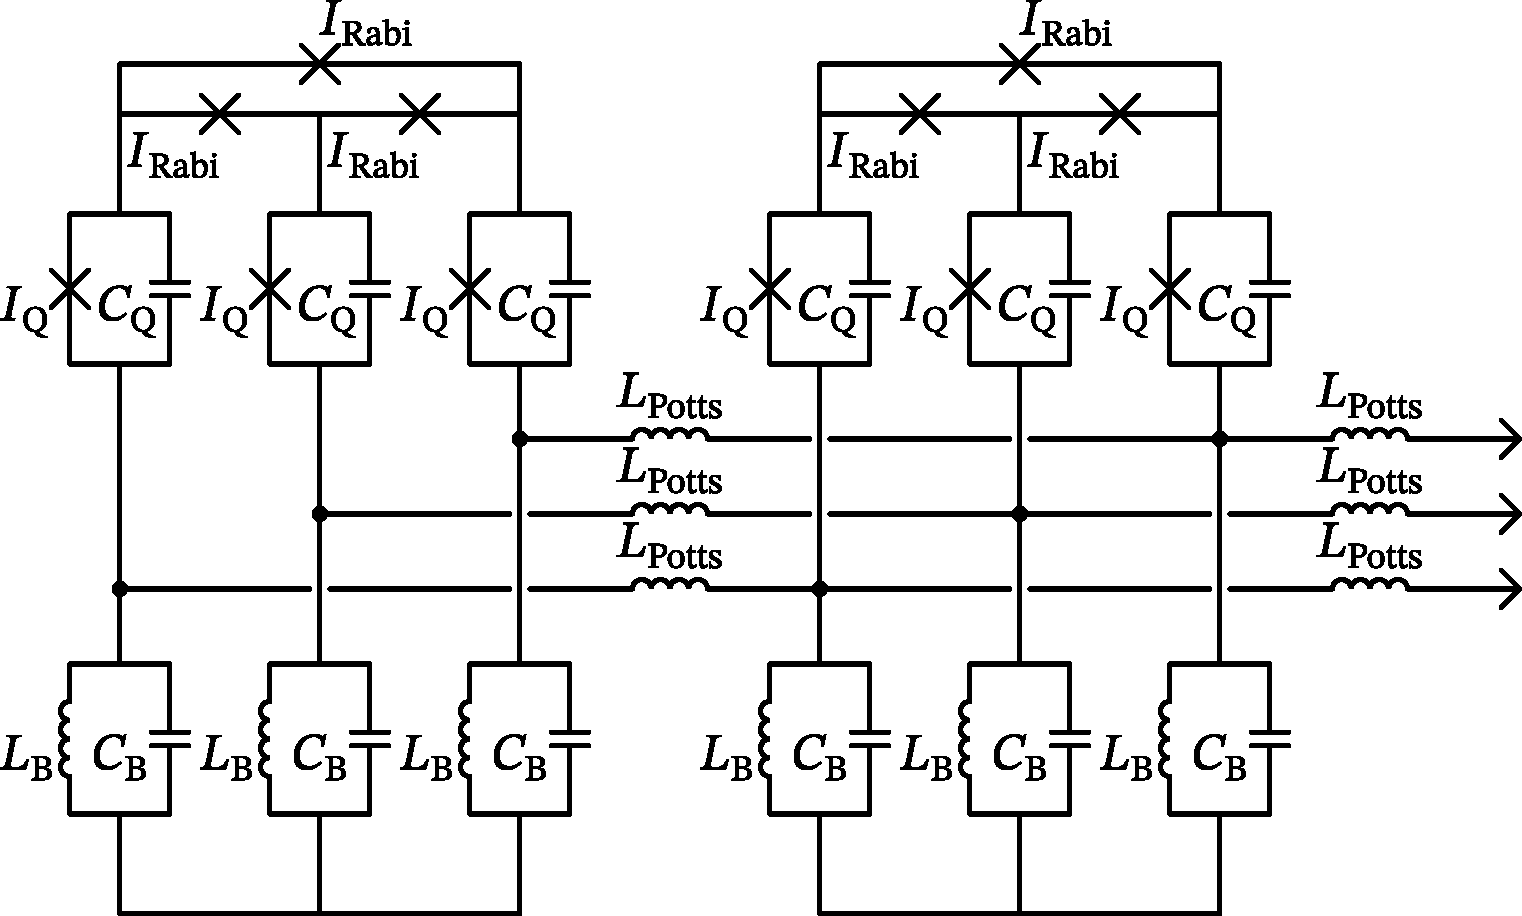
\includegraphics[width=\linewidth]{pics/SC_Potts_circuit_new_svg-tex.pdf}
    \caption{Superconducting circuit implementation of the Potts model. The circuit is described by the Hamiltonian (\ref{coupled-rabi}). Subscript ``B'' denote elements corresponding to boson degrees of freedom; subscript ``Q'' denote qubit elements; subscript ``Rabi'' denote elements responsible for interaction in qubit-boson ring; subscript ``Potts'' denote elements responsible for interaction in Potts model.}
    \label{fig:superconducting-potts}
\end{figure}

It is straightforward to implement the Potts model based on superconducting circuits. We consider a chain of superconducting circuits depicted in Fig. \ref{fig:superconducting-Rabi}. Next, we need to couple the neighbor Rabi models with a boson hopping term to get the Hamiltonian (\ref{coupled-rabi}). To do it, we couple the neighbor Rabi models using inductors (Fig. \ref{fig:superconducting-potts}). Although capacitive coupling is more common, here it induces unwanted  all-to-all coupling.

On the other hand, the inductor coupling leads us to the hopping term we want. First of all, the Hamiltonian terms corresponding to the inductors are:
\begin{equation}
\begin{aligned}
    &\hat V_{\text{Potts},n} = \frac{1}{2L_{\text{Potts}}} (\hat \phi_{n+1} - \hat \phi_n)^2 = \frac{\hat \phi_n^2 + \hat \phi_{n+1}^2}{2L_{\text{Potts}}} \\
    &+ \frac{\hat a^{\dagger}_n \hat a^{\dagger}_{n+1} + \hat a^{\dagger}_n \hat a_{n+1} + \hat a_n \hat a^{\dagger}_{n+1} + \hat a_n \hat a_{n+1}}{L_{\text{Potts}}C_{\text{B}}\Omega_{QB}} 
\end{aligned}
\end{equation}
where we expressed the flux operator through the creation/annihilation operators $\hat \phi_n = (\hat a_n + \hat a_n^{\dagger})/\sqrt{2C_{\text{B}} \Omega_{QB}}$.

We ignore the $ \hat \phi_n^2 $ and $ \hat \phi_{n+1}^2 $ terms because they simply renormalize the Rabi model parameters. Additionally, the inductor coupling produces undesired terms $\hat a^{\dagger}_n \hat a^{\dagger}_{n+1}$ and $\hat a_n \hat a_{n+1}$. However, we can use Rotating Wave Approximation (RWA) to eliminate them. For the RWA to be applicable, we need $\Omega_{QB} = \sqrt{L_{\text{B}} C_{\text{B}}} \gg (L_{\text{Potts}} C_{\text{B}} \Omega_{QB})^{-1}$. After RWA we are left with the hopping term between the boson modes of the neighbor Rabi model. Consequently, in line with Sec. \ref{theoretical-potts} the superconducting circuit in question is modeled by the Potts model. The coupling parameters of the resulting Pottsd model could be expressed through the circuit parameters:
\begin{equation}
\begin{aligned}
    &f_{\text{Potts}} = \frac{I_{\text{Rabi}}}{2} \exp\left(-\frac{1}{2}\sqrt{\frac{L_{\text{B}}}{C_{\text{B}}}}\right), \\
    &J_{\text{Potts}} = \frac{1}{2L_{\text{Potts}}}\sqrt{\frac{L_{\text{B}}}{C_{\text{B}}}}. 
\end{aligned}
\end{equation}


\subsection{Coupled optomechanical \texorpdfstring{$\Zthree$}{Z3} Rabi models}

\begin{figure}[t]
    \centering
    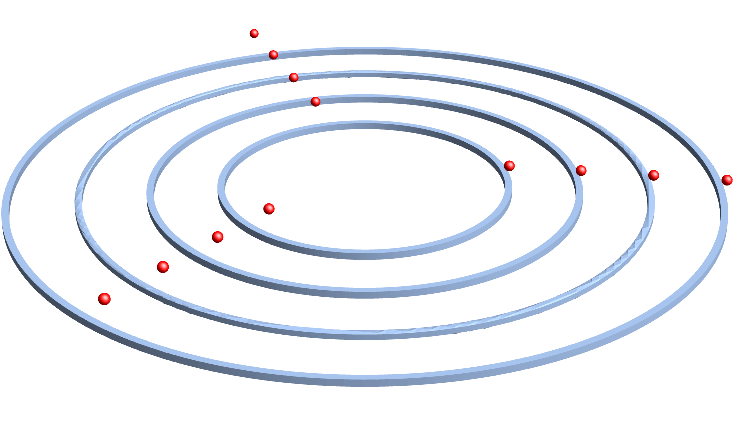
\includegraphics[width = 0.8 \linewidth]{pics/optomechanical_Potts_pic.pdf}
    \caption{Schematic illustration of the optomechanical (OM) implementation of the Potts model. It consists of several concentric OM implementations of the Rabi model, i.e., several concentric cyclic chiral waveguide and three trapped ions on top of each waveguide.}
    \label{fig:optomechanical-potts}
\end{figure}

We can repeat the same procedure for the optomechanical system. However, it is a bit more peculiar, because of the circular waveguide in the optomechanical Rabi model. To build the optomechanical $\Zthree$ Potts model we arrange the optomechanical $\Zthree$ Rabi model concentrically (see Fig. \ref{fig:optomechanical-potts}). On the one hand, the radius of the waveguide does not affect the parameters of the model, on the other hand, placing the ions of the neighbor Rabi models close to each other creates phonon-phonon interaction through the ion Coulomb interaction \cite{schneider_experimental_2012,timm_dynamics_2023}. The phonon-phonon interaction between the neighboring Rabi models leads to the Hamiltonian (\ref{coupled-rabi}) and consequently to the $\Zthree$ Potts model as described before.


\subsection{Chiral Potts model and parafermions}


\begin{figure*}[t]
    \captionsetup[subfloat]{captionskip=-135pt} %%Moving captions on top
    \centering
    \subfloat[]{
         \centering
         %%\caption{}
        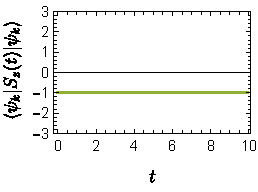
\includegraphics[width=0.32\linewidth]{pics/Spin_correlators_1.pdf}
         \label{fig:1st-spin-correlator}}
    \subfloat[]{
         \centering
        %%\caption{ }
        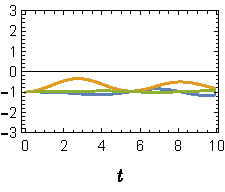
\includegraphics[width=0.274\linewidth]{pics/Spin_correlators_2.pdf}
         \label{fig:2nd-spin-correlator}}
    \subfloat[]{
         \centering
        %%\caption{}
        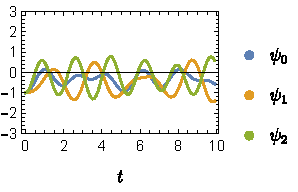
\includegraphics[width=0.37\linewidth]{pics/Spin_correlators_3.pdf}
         \label{fig:3rd-spin-correlator}}
    \caption{Time dependence of the total spin excitation operator. To illustrate robustness of the Rabi model implementation with the respect of disorder (\ref{rabi-breaking-disorder}) we plotted $\langle S_z(t) \rangle$. The standard variance of the disorder $\Delta_j$ equals for plot a) 0.1; b) 0.3; c) 1.}
    \label{fig:spin-excitation-plot}
\end{figure*}


In this subsection, we want to briefly overview the chiral Potts model. It is a generalization of the ordinary Potts model that has a chiral nearest-neighbour interaction:
\begin{equation}
\label{chiral-potts-hamiltonian}
\begin{aligned}
    H_{\text{chPotts}} = &f'\sum_{n=1}^L (e^{i\phi'} Z_n + e^{-i\phi'} Z_n^{\dagger}) \\
    &+ J' \sum (e^{i\theta'} X_n X_{n+1}^{\dagger} + e^{-i\theta'} X_n^{\dagger} X_{n+1}).
\end{aligned}
\end{equation}
It is simply the Potts model (\ref{potts-hamiltonian}) with a complex parameter $J'$. 

The chiral Potts model exhibits richer physics compared to the ordinary one. In particular, it can host parafermion physics. We discuss it more below, but first, we need to discuss how to obtain this chiral interaction, because it is quite challenging.

As mentioned earlier, the interaction parameter $J'$ originates from the neighbor $\Zthree$ Rabi models boson interaction. Hence, if we want to obtain the chiral Potts model, we have to obtain a chiral boson-hopping term. The full technical discussion of this topic is outside of this paper's scope. However, we want to mention that recently a way to obtain the chiral boson hopping was proposed in \cite{bermudez_synthetic_2011}, and we assume that it could be adapted to our system.

For the Potts system a certain generalization of the Jordan-Wigner transformation exists. It is called the Fradkin-Kadanoff (FK) transformation \cite{fradkin_disorder_1980}, and it allows us to rewrite $X_j, \, Z_j$ in terms of parafermions:
\begin{equation}
\Gamma_j = \prod\limits_{k<j} Z_k X_j , \quad \Delta_j = \prod\limits_{k\le j} Z_k X_j.
\end{equation}
Here $\Gamma_j, \, \Delta_j$ are parafermion operators with a parafermion commutation relation: $\Gamma_j \Gamma_k = \omega^{\sgn(j-k)} \Gamma_k \Gamma_j, \, \Delta_j \Delta_k = \omega^{\sgn(j-k)} \Delta_k \Delta_j$, and finally $\Gamma_j \Delta_k = \omega^{\sgn(j-k)} \Delta_k \Gamma_j$.

Using the FK transformation, it is easy to show that the Potts model is equivalent to a parafermion chain. The only problem is that FK transformation is not local. In terms of parafermion operators, the chiral Potts model Hamiltonian (\ref{chiral-potts-hamiltonian}) looks like 


\begin{equation}
\begin{aligned}
    H_{\text{chPotts}} = &f' \sum \left( e^{i\phi'} \Gamma_j \Delta_j^{\dagger} + e^{-i\phi'} \Delta_j \Gamma_j^{\dagger}\right) \\
    &+J' \sum \left(e^{i\theta'} \Delta_j \Gamma_{j+1}^{\dagger} + e^{-i\theta'} \Gamma_{j+1} \Delta_j^{\dagger}\right)
\end{aligned}
\end{equation}



On the other hand, it is known that parafermion chain has a phase with a parafermion edge mode  \cite{fendley_parafermionic_2012}:
\begin{equation}
\Gamma_{\text{edge}} = \Gamma_1 + \frac{f'}{J' \sin(3\theta')} \mathcal{O} + \dots
\end{equation}

Unfortunately, after the parafermion edge mode is not localized on the edged after FK transformation. As a result, we do not have an actual topological phase in the chiral Potts model. But we believe that it still holds an importance because it allows us to simulate a parafermion chain.


\section{Disorder in the superconducting implementation}
\subsection{Disorder breaking the total qubit excitation number conservation}


First, while discussing the effect of the disorder on the qubit-boson ring (\ref{physical-hamiltonian}), we need to consider a term that breaks the conservation of the total excitation number of qubits $\hat S^z$. This conservation law is broken by the Zeeman terms being not perfectly aligned with $\hat z$ direction:
\begin{equation}
    \hat H_{QB,\text{dis}} = \hat H_{QB} + \sum_{j=1}^3 \Delta_j \sigma_j^x.
\end{equation}
As explained in App. \ref{charge-qubit}, $\Delta_j$ being equal to zero for qubit-boson ring based on superconducting circuits relies on the fine-tuning of the SQUID magnetic field. Therefore, in a realistic setting we unavoidably are going to have non-zero $\Delta_j = I_{Q,1}\sin(\Delta \Phi_j)$.

As a result, we have $[\hat H_{QB,\text{dis}}, \hat S^z] \neq 0 $. Unfortunately, it breaks the derivation of the Rabi model. However, assuming that the disorder is considerably smaller then other parameters in the Hamiltonian, we can still hope that the dynamics is approximately governed by the Rabi model. Because an analytic estimate is cumbersome, we performed numerical simulations of the qubit–boson ring. The results could be seen on Fig. \ref{fig:spin-excitation-plot}. The simulation shows that for the small disorder the qubit-boson ring stays around the single excitation subspace $\mathcal{H}_1$ because $\langle \hat S^z \rangle(t) \approx 1$. We speculate that it happens because the spins precess around $\langle \hat S^z \rangle = 1$.


\subsection{Disorder breaking \texorpdfstring{$\Zthree$}{Z3} symmetry}

Now, assuming that the total number of qubit excitations is conserved, we would like to investigate how the coordinate dependence of the parameter in the qubit-boson ring influences the resulting Rabi model. The spatial non-homogeneity obviously breaks the $\Zthree$ symmetry. However, we want to find the explicit symmetry-breaking term.
\begin{equation}
\label{rabi-breaking-disorder}
\begin{aligned}
  \hat H_{QB}' &= \sum_j \epsilon_{j} \sigma_j^z + \sum_j \Omega_j \hat a^{\dagger}_j \hat a_j  \\
  &+ \sum_j g_{j,j+1} \left[\sigma_j^+ \sigma_{j+1}^- e^{i (\hat x_j - \hat x_{j+1})} +\text{h.c}\right]
\end{aligned}
\end{equation}
where we have
\begin{equation}
\begin{aligned}
    &\epsilon_j = \frac{\delta_j}{2 C_{Q,j}},\,
    \Omega_{QB,j} = \left(L_{\text{B},j}C_{\text{B},j}\right)^{-1/2}, \\
    &g_{j,j+1} = \frac{I_{\text{Rabi},j}}{2}.
\end{aligned}
\end{equation}

For brevity, we decompose the coupling parameters into a homogeneous part and a disorder: $\epsilon_j = \epsilon + \Delta \epsilon_j$, $\Omega_j = \Omega + \Delta \Omega_j$, $g_{j,j+1} = g + \Delta g_{j,j+1}$, where we assume that the disorder averaged over the coordinate is zero: $\sum_j \Delta \epsilon_j =  \sum_j \Delta \Omega_j = \sum_j \Delta g_{j,j+1} =0$. We can always achieve this by adjusting the homogeneous coupling.

Then the single-excitation sector is going to be described by
\begin{equation}
\begin{aligned}
    &\hat H_{\text{2 Rabi}}' = \hat H_{\text{2 Rabi}} + \epsilon(2) X \\
    &+\epsilon(1)  X^{\dagger} + (X + X^{\dagger}) \sum\limits_{k=1}^2 \Delta g(k) Z^k\\
    &+ \Omega(1) \sum\limits_{k=0}^2 \hat a^{\dagger}(k+1) \hat a(k) + \Omega(2) \sum\limits_{k=0}^2 \hat a^{\dagger}(k) \hat a(k+1) \\
    &+ \sum\limits_{l=1}^2 \frac{\Omega^{3/2}(l)}{2^{3/2}} \sum\limits_{k=0}^2 (\hat a(k+l) + \hat a^{\dagger}(-k-l)) Z^k.
\end{aligned}
\end{equation}

Due to the disorder the first boson mode does not decouple anymore. However, the structure of threefold cat state should be still conserved for small disorder. 


\section{Conclusion}

We have explored $\Zthree$-symmetric models, with a particular focus on the $\Zthree$ Rabi model and its variations. By employing a canonical transformation, we successfully derived the spectrum of these models, revealing that the three lowest eigenstates correspond to distinct threefold cat states, a feature interesting from several perspectives. We derived an analytical expression for the Wigner quasi-probability function of the threefold cat state and used it to better understand the structure of the cat states.

We also introduced a hierarchy of $\Zthree$-symmetric systems. In the qubit-boson ring, the $\Zthree$ symmetry appears as a discrete rotational symmetry, whereas in the Rabi model, a specific sector of the qubit-boson ring, the symmetry acts as an internal one. This internal symmetry also exists in the $\Zthree$ Potts model, which we constructed by coupling multiple $\Zthree$ Rabi models.

Our main goal was to suggest a way towards an experimental realization of the $\Zthree$ Rabi and Potts models. We believe that the proposed superconducting circuit should be feasible to implement. However, this approach does not have to be restricted only to the superconducting circuit platform. For example, we believe that a similar strategy work for the spin-qubit systems. Though, this remains a topic for a future research.

More broadly, our work highlights the intriguing potential of $\Zn$-symmetric systems within condensed matter physics. These systems present a fertile ground for discovering novel quantum phenomena, many of which are yet to be fully understood or described. We believe that the further investigation into these models reveals new insights and advance our understanding of symmetry in quantum systems.

\section*{Acknowledgments} 

We thank Daria Kalacheva, Henry Legg, Katharina Laubscher, and Ilia Luchnikov for fruitful discussions and useful comments. This work was supported as a part of NCCR SPIN, a National Centre of Competence in Research, funded by the Swiss National Science Foundation (grant number 225153). This work has received funding from the Swiss State Secretariat for Education, Research and Innovation (SERI) under contract number M822.00078.


\appendix

\section{Generalisation to an arbitrary interaction matrix}
\label{arbitrary-interaction-summary}

For completeness we summarise how the above derivation extends to a QB ring
with an arbitrary $\Zthree$--symmetric interaction matrix~$A$.  The starting
Hamiltonian is
\begin{equation}
\label{arbitary-interaction-hamiltonian}
  \begin{aligned}
    \hat H_{\text{gen}} &= \epsilon \sum_{j=1}^{3} \sigma_j^z
      + \Omega \sum_{j=1}^{3} \hat a_j^{\dagger} \hat a_j + \hat V_{\text{gen}},
      \\
    \hat V_{\text{gen}} &= g \sum_{j,k} A_{jk}
      \sigma_j^{+} \sigma_k^{-} e^{ i ( \hat x_j - \hat x_k ) },
  \end{aligned}
\end{equation}
with $A^{\dagger}=A$.  The same sequence of steps---momentum translation $S$,
Fourier transform, and restriction to $\mathcal H_{\text{QB},1}$---again leads
to the two--mode Hamiltonian\footnote{An additional basis change might be
required to diagonalise the purely spin term.}
\eqref{effective-rabi}, now with $gA$ replacing $g(Z+Z^{\dagger})$.  Hence any
interaction matrix compatible with $\Zthree$ symmetry can be mapped onto the
canonical Rabi model.  The parameter correspondence reads
\begin{equation}
  \Omega_R = \Omega, \qquad \lambda = \sqrt{ \frac{\Omega}{6 m} }.
\end{equation}

In the superconducting implementation one has $A = X + X^{\dagger}$, thereby
recovering the special case treated above.  The optomechanical realisation
gives rise to a different Hermitian $A$ but follows exactly the same logic.



\section{Charge qubit for the \texorpdfstring{$\Zthree$}{Z3} Rabi model}
\label{charge-qubit}



The Cooper Pair Box (CPB) qubit is the most well-known type of charge qubit. However, it is not suitable for our purposes because its eigenstates are not charge states but their symmetric/antisymmetric combinations. Its Hamiltonian is proportional to $\sigma^x$. But in this case, the qubit chain Hamiltonian does not commute with total number of qubit excitations operator $S^z$.

Hence, we need another type of a charge qubit. Considering that the $\sigma^x$ term in the Hamiltonian arises from the JJ term the natural idea is to get rid of the JJ and consider a purely capacitor qubit. Although theoretically suitable for our purposes, without the JJ the charge qubit is very sensitive to noise. Therefore, it is not a realistic approach.

Consequently, we want two things simultaneously: Hamiltonian proportional to $\sigma^z$ in charge basis and JJ to fight noise. The solution turns out to be a higher harmonic Josephson junction. Usually it is neglected, but the JJ Hamiltonian always include higher harmonics as well
\begin{equation}
    \hat H_{JJ} = E_{J,1} \cos{\hat \phi} + E_{J,2} \cos{2\hat \phi} + \dots,
\end{equation}
where $\phi$ is the superconducting phase.

In practice, the higher harmonics are usually considerably weaker $E_{J,2} \ll E_{J,1}$. But if we were to eliminate the first harmonic completely, then we would be left with the second harmonic. The second harmonic, on the one hand, can help to supress the noise and, on the other hand, does not appear in the qubit Hamiltonian:
\begin{equation}
    \cos{2\hat \phi}\bigg|_{\mathcal{V}} = \frac{1}{2}\left(e^{2i\hat\phi} + e^{-2i\hat \phi}\right)\bigg|_{\mathcal{V}}=\frac{1}{2}\left((\sigma^+)^2 + (\sigma^-)^2\right) =0
\end{equation}

To eliminate the first harmonic, we can use a Superconducting Quantum Interference Device (SQUID) \cite{valentini_parityconserving_2024}. If the magnetic flux through the SQUID is tuned to $\Phi = \pi$, then the SQUID Hamiltonian looks like:
\begin{equation}
\begin{aligned}
    \hat H_{squid} = &I_{Q,1} \cos(\hat \phi) + I_{Q,2} \cos(2\hat \phi) + I_{Q,1} \cos(\hat \phi + \pi) \\
    &+ I_{Q,2} \cos(2\hat \phi + 2\pi) = 2 I_{Q,2} \cos(2\hat \phi).
\end{aligned}
\end{equation}
As a result, only the second harmonic is left.

Consequently, we can construct a qubit based on the second-harmonic JJ (see Fig. \ref{fig:second-harmonic-qubit}). It is described by the Hamiltonian:
\begin{equation}
\label{second-harmonic-qubit}
    \hat H = \frac{1}{2C_Q} (\hat n - n_0)^2 + 2 I_{Q,2} \cos(2\hat\phi)
\end{equation}
If we tune $n_0$ a bit off 1/2: $n_0 = 0.5 - \delta$, then the qubit Hamiltonian looks like:
\begin{equation}
    \hat H_{\text{qubit}} = \frac{\delta}{2 C_Q} \sigma_z.
\end{equation}
Hence, we obtained the qubit Hamiltonian we wanted. Here we consider $\frac{1}{2C} \gg 2 E_{J,2}$ as usual for charge qubits.

To conclude, the charge qubit we have in mind consists of a capacitor and the second-harmonic JJ. One can think of it as a certain generalization of a Cooper Pair Box qubit. In this appendix, we only briefly described its blueprint to give additional substance to the proposal in Sec. \ref{superconducting-implementation}.




\bibliography{references}

\end{document}
